\documentclass[11pt]{article}
\usepackage{times}
\usepackage{amsmath,amsthm,amssymb,setspace,enumitem,epsfig,titlesec,verbatim,color,array,eurosym,multirow}
\usepackage[sort&compress]{natbib}
\usepackage[footnotesize,bf]{caption}
\usepackage[top=2.2cm,left=2.4cm,right=2.4cm,bottom=3cm]{geometry}
\smallskip % Erlaubt kleine Abstaende zwischen Paragraphen, falls es dem Seitenlayout hilft
\renewcommand{\baselinestretch}{1.3}
\newcommand{\R}{\mathbb{R}}

\definecolor{darkblue}{rgb}{0,0,.8}
\definecolor{darkgreen}{rgb}{0,0.5,0.1}
\newcommand{\matlabfunc}[1]{\textcolor{darkblue}{#1}}
\newcommand{\matlabcomment}[1]{\textcolor{darkgreen}{#1}}
\newcommand{\christian}[1]{\textcolor{blue}{\textbf{CH}: #1}}
\newcommand{\alex}[1]{\textcolor{red}{\textbf{AL}: #1}}

%% Adding shortcut commands to refer to our figures %%
\newcommand{\FigEvoProc}{{\bf Fig.~1}}
\newcommand{\FigInvAnalysis}{{\bf Fig.~2}}
\newcommand{\FigResultsOverPara}{{\bf Fig.~3}}


\titleformat{\section}{\sffamily \fontsize{12}{14}\bfseries}{\thesection}{1em}{}
\titleformat{\subsection}{\sffamily \fontsize{11.5}{11.5}\bfseries}{\thesubsection}{1em}{}


\newtheoremstyle{plainCl1}% name
{9pt}%      Space above, empty = 'usual value'
{9pt}%      Space below
{\it}% 	   Body font
{}%         Indent amount (empty = no indent, \parindent = para indent)
{\bfseries}% Thm head font
{.}%        Punctuation after thm head
{0.2cm}% Space after thm head: \newline = linebreak
{}%         Thm head spec

\newtheoremstyle{plainCl2}% name
{9pt}%      Space above, empty = 'usual value'
{9pt}%      Space below
{\it}% 	   Body font
{}%         Indent amount (empty = no indent, \parindent = para indent)
{\bfseries}% Thm head font
{$'$.}%        Punctuation after thm head
{0.2cm}% Space after thm head: \newline = linebreak
{}%         Thm head spec


\theoremstyle{plainCl1}
\newtheorem{Claim}{Claim}
\newtheorem{Thm}{Theorem}
\newtheorem{Prop}{Proposition}
\newtheorem*{Lem}{Lemma}
\newtheorem{Cor}{Corollary}
\newtheorem*{Def}{Definition}

\theoremstyle{plainCl2}
\newtheorem{Claim2}{Claim}

\title{\begin{center}
\bf  \sffamily \LARGE Prisoner's dilemma with stochastic payoffs\\[-1cm]
\end{center}}
\date{}
\author{}

\begin{document}
\maketitle

\section{Introduction}

In the evolutionary dynamics literature it is common that the expected payoffs are
used in order to estimate individuals payoffs, and as a result, their fixation
probabilities.

The aim of this work is to understand the effect of the payoffs on the evolution
of the population. More specifically, this works evaluates the evolution for differently
calculated stochastic payoffs.

\section{Model}

The Prisoner's Dilemma (PD) is a two player no-cooperative game. The players
simultaneously and independently make a decision to Cooperate (C) or to defect
(D). The payoffs for both players depend on their actions and the actions of
their opponents. More specifically, the payoffs are given by:

\begin{equation}\label{eq:pd_normal_form}
    \begin{pmatrix}
        R & S  \\
        T & P
    \end{pmatrix}
\end{equation}

The payoffs, \((R, P, S, T)\), are constrained by \(T > R > P > S\) and \(2R > T + S\).
A special case of the PD is that of the donation game where the matrix~(\ref{eq:pd_normal_form})
is now written as:

A special case is the donation game,” where each player can cooperate by providing 
a benefit \(b\) to the other player at their cost \(c\), with \(0 < c < b\).
Then, \(T=b, R=b-c, S=-c, P=0\), and matrix~(\ref{eq:pd_normal_form}) is give by:

\begin{equation}\label{eq:donation_normal_form}
    \begin{pmatrix}
        b-c & -c  \\
        b & 0
    \end{pmatrix}
\end{equation}

where \(c\) is the cost inflicted to an individual for cooperating and \(b\) is
the benefit.

The game becomes more interesting once repetition is taken into account, and
now te history of play is taken into account when making decisions. The iterated
form of the game is called the Iterated Prisoner's Dilemma (IPD). There are other
two players repeated games such as the Snowdrift game, Harmony and the Stag Hunt
game. These games are also taken into account in the numerical simulations section.

The space of strategies is infinite in the IPD. In this work we assume that
the individuals of our population can only follow a reactive strategy.

Reactive strategy are a set of memory-one strategies that only take into account
the previous action of the opponent. An example of a reactive strategy is Tit
For Tat. Reactive strategies can be written explicitly as a vector \(\in
\R_{3}\). More specifically a reactive strategy \(s\) is given by \(s=(y, p,
q)\) where \(y\) is the probability that the strategy opens with a cooperation
and \(p, q\) are the probabilities that the strategy cooperates given that the
opponent cooperated and defected equivalently.

Two players with reactive strategies takes the form of a Markov chain
with four possible states CC, CD, DC, DD (the possible outcomes of each round).
Given two reactive strategies \(s_{1}=(y_{1}, p_{1}, q_{1})\) and 
\(s_{2}=(y_{2}, p_{2}, q_{2})\), the transition matrix \(M\) of this Markov chain
is given by:

\begin{equation}
    M = \left[\begin{matrix} p_{1} p_{2} & p_{1} \left(1 - p_{2}\right) & p_{2} \left(1 - p_{1}\right) & \left(1 - p_{1}\right) \left(1 - p_{2}\right)\\
    p_{2} q_{1} & q_{1} \left(1 - p_{2}\right) & p_{2} \left(1 - q_{1}\right) & \left(1 - p_{2}\right) \left(1 - q_{1}\right)\\
    p_{1} q_{2} & p_{1} \left(1 - q_{2}\right) & q_{2} \left(1 - p_{1}\right) & \left(1 - p_{1}\right) \left(1 - q_{2}\right)\\
    q_{1} q_{2} & q_{1} \left(1 - q_{2}\right) & q_{2} \left(1 - q_{1}\right) & \left(1 - q_{1}\right) \left(1 - q_{2}\right)\end{matrix}\right]
\end{equation}

The long run steady state probability
vector \(\mathbf{v}\), which is the solution to \(\mathbf{v} M = \mathbf{v}\), can be
combined with the payoff of matrix (\ref{eq:pd_normal_form}) to give the expected
payoffs for each player. More specifically, the payoffs for a reactive
strategy \(s_1\) against an opponent \(s_2\), is given by:

\begin{equation}
    \mathbf{v}(s_1, s_2) \cdot u
\end{equation}

The basic setup is a population of \(N\)
individuals, where \(N\) is even, and where mutations are sufficiently rare such
that at any point in time at most two different strategies are present in the
population. Suppose there are \(N - k\) players who use the strategy \(s_{1}=(y_{1},
p_{1}, q_{1})\), whereas \(k\) players use the strategy \(s_{2}=(y_{2}, p_{2},
q_{2})\). We refer to these two player types as ‘residents’ and ‘mutants’,
respectively.

Each step of the evolutionary process consists of two stages, a game stage and
an updating stage. In the game stage, each player is randomly matched with some
other player in the population to interact in one instance of the repeated
prisoner's dilemma. In the updating stage, two players are randomly drawn from
the population, a `learner' and a `role model'. Given that the learner's payoff
in the last round is $u_L\!\in\! \mathcal{U}$ and that the role model's last
round's payoff $u_M\!\in\! \mathcal{U}$, we assume the learner adopts the role
model's strategy with probability 

\begin{equation} \label{Eq:rho}
\rho(u_L, u_M) = \frac{1}{1\!+\!\exp\big[ \!-\!\beta (u_M\!-\!u_L) \big]}. 
\end{equation}

The parameter $\beta\!\ge\!0$ corresponds to the strength of selection.

We iterate this basic evolutionary step until either the mutant strategy goes
extinct, or until it fixes in the population (in which case the mutant strategy
becomes the new resident strategy). After either outcome, we introduce a new
mutant strategy $S'_2\!=\!(y_2',p_2',q_2')$ (uniformly chosen from all reactive
strategies at random), and we set the number of mutants to $k\!=\!1$. This
process of mutation and fixation/extinction is then iterated many times. 

We compare this process for stochastic payoff evaluation with the analogous
process where players update their strategies with respect to their {\it
expected} payoffs,
\begin{equation} \label{Eq:ExpPay}
\begin{array}{lcrcr}
\displaystyle \pi_1	&=	&\displaystyle \frac{N\!-\!k\!-\!1}{N-1}\cdot \langle\mathbf{v}(S_1,S_1),\mathbf{u}\rangle	&+	&\displaystyle\frac{k}{N-1}\cdot \langle\mathbf{v}(S_1,S_2),\mathbf{u}\rangle,\\[0.5cm]
\displaystyle \pi_2	&=	&\displaystyle\frac{N-k}{N-1}\cdot \langle\mathbf{v}(S_2,S_1),\mathbf{u}\rangle&+	&\displaystyle\frac{k-1}{N-1}\cdot \langle\mathbf{v}(S_2,S_2),\mathbf{u}\rangle.\\
\end{array}
\end{equation}
In the limit of no discounting, $\delta\!\rightarrow\! 1$, this process based on
expected payoffs has been considered in~\cite{imhof:prsb:2010}. 



% \begin{equation}\label{eq:transition_matrix}
%     \resizebox{.5\hsize}{!}{$\input{tex/m_matrix.tex}$}
% \end{equation}


% \begin{equation}\label{eq:press_dyson_utility}
%     u_q(p) = v \cdot (R, S, T, P).
% \end{equation}

\section{Games dynamics between reactive strategies}

Consider two players with reactive strategies $S_1\!=\!(y_1, p_1, q_1$) and $S_2\!=\!(y_2,p_2,q_2)$ who interact in a repeated prisoner's dilemma with continuation probability $\delta$. We consider the vector 
\begin{equation}
\mathbf{v}(S_1,S_2)\!=\!\Big(v_{R}(S_1,S_2),v_{S}(S_1,S_2),v_{T}(S_1,S_2),v_{P}(S_1,S_2)\Big)\!:=\!(1\!-\!\delta)\mathbf{v_0}(I_4-\delta M)^{-1}.
\end{equation}
Here, $\mathbf{v_0}$ denotes the expected distribution of the four outcomes in the very first round, $I_4$ is the $4\!\times\!4$ identity matrix, and $M$ is the transition matrix of the Markov chain. 
The entries of $\mathbf{v}$ can be calculated explicitly,
\begin{equation} \label{Eq:LastRound}
\setlength{\arraycolsep}{1pt}
\begin{array}{rcl}

v_{R}(S_1,S_2)	&=	&\displaystyle (1\!-\!\delta)\frac{y_1y_2}{1\!-\!\delta^2 r_1 r_2}+\delta \frac{\Big(q_1+r_1\big((1\!-\!\delta)y_2+\delta q_2\big)\Big) \Big(q_2+r_2\big((1\!-\!\delta)y_1+\delta q_1\big)\Big)}
{\displaystyle(1\!-\!\delta r_1r_2)(1\!-\!\delta^2 r_1 r_2)},\\[1cm]

v_{S}(S_1,S_2)	&=	&\displaystyle (1\!-\!\delta)\frac{y_1\bar{y}_2}{1\!-\!\delta^2 r_1 r_2}+\delta \frac{\Big(q_1+r_1\big((1\!-\!\delta)y_2+\delta q_2\big)\Big) \Big(\bar{q}_2+\bar{r}_2\big((1\!-\!\delta)y_1+\delta p_1\big)\Big)}
{\displaystyle(1\!-\!\delta r_1r_2)(1\!-\!\delta^2 r_1 r_2)},\\[1cm]

v_{T}(S_1,S_2)	&=	&\displaystyle (1\!-\!\delta)\frac{\bar{y}_1y_2}{1\!-\!\delta^2 r_1 r_2}+\delta \frac{\Big(\bar{q}_1+\bar{r}_1\big((1\!-\!\delta)y_2+\delta p_2\big)\Big) \Big(q_2+r_2\big((1\!-\!\delta)y_1+\delta q_1\big)\Big)}
{\displaystyle(1\!-\!\delta r_1r_2)(1\!-\!\delta^2 r_1 r_2)},\\[1cm]

v_{P}(S_1,S_2)	&=	&\displaystyle (1\!-\!\delta)\frac{\bar{y}_1\bar{y}_2}{1\!-\!\delta^2 r_1 r_2}+\delta \frac{\Big(\bar{q}_1+\bar{r}_1\big((1\!-\!\delta)y_2+\delta p_2\big)\Big) \Big(\bar{q}_2+\bar{r}_2\big((1\!-\!\delta)y_1+\delta p_1\big)\Big)}
{\displaystyle(1\!-\!\delta r_1r_2)(1\!-\!\delta^2 r_1 r_2)}.

%x_1(S_1,S_2)&=&\displaystyle\frac{(1\!-\!\delta)y_1+\delta\Big(q_1+r_1\big((1\!-\!\delta)y_2+\delta q_2\big)\Big)}{1-\delta^2r_1r_2}\\[0.7cm]
%x_2(S_1,S_2)&=&\displaystyle\frac{(1\!-\!\delta)y_2+\delta\Big(q_2+r_2\big((1\!-\!\delta)y_1+\delta q_1\big)\Big)}{1-\delta^2r_1r_2}.\\
\end{array}
\end{equation}
In these expressions, we have used the notation $r_i:=p_i\!-\!q_i$, $\bar{y}_i\!=\!1\!-\!y_i$, $\bar{q}_i:=1\!-\!q_i$, and $\bar{r}_i:=\bar{p}_i\!-\!\bar{q}_i=-r_i$ for $i\!\in\!\{1,2\}$. Let $\mathcal{U}=\{R,S,T,P\}$ denote the set of feasible payoffs in each round, and let $\mathbf{u}\!=\!(R,S,T,P)$ be the corresponding payoff vector. Then one can show the following result.

\begin{Prop}
Consider a repeated prisoner's dilemma between players with reactive strategies $S_1\!=\!(y_1, p_1, q_1$)  and $S_2\!=\!(y_2,p_2,q_2)$ respectively. Then the probability that the $S_1$ player receives the payoff $u\!\in\! \mathcal{U}$ in the very last round of the game is given by $v_{u}(S_1,S_2)$, as given by Eq.~(\ref{Eq:LastRound}). 
\end{Prop}


\section{Pairwise imitation dynamics under stochastic payoff evaluation}

\subsection{Basic setup} \label{Sec:BasicSetup}
In the following we consider a population of size $N$, where $N$ is even. We assume mutations are sufficiently rare such that at any point in time at most two different strategies are present in the population. Suppose there are $N\!-\!k$ players who use the strategy $S_1\!=\!(y_1,p_1,q_1)$, whereas $k$ players use the strategy $S_2\!=\!(y_2,p_2,q_2)$. We refer to these two player types as `residents' and `mutants', respectively. 

Each step of the evolutionary process consists of two stages, a game stage and an updating stage. In the game stage, each player is randomly matched with some other player in the population to interact in one instance of the repeated prisoner's dilemma. 
In the updating stage, two players are randomly drawn from the population, a `learner' and a `role model'. Given that the learner's payoff in the last round is $u_L\!\in\! \mathcal{U}$ and that the role model's last round's payoff $u_M\!\in\! \mathcal{U}$, we assume the learner adopts the role model's strategy with probability 
\begin{equation} \label{Eq:rho}
\rho(u_L, u_M) = \frac{1}{1\!+\!\exp\big[ \!-\!\beta (u_M\!-\!u_L) \big]}. 
\end{equation}
The parameter $\beta\!\ge\!0$ corresponds to the strength of selection.

We iterate this basic evolutionary step until either the mutant strategy goes extinct, or until it fixes in the population (in which case the mutant strategy becomes the new resident strategy). After either outcome, we introduce a new mutant strategy $S'_2\!=\!(y_2',p_2',q_2')$ (uniformly chosen from all reactive strategies at random), and we set the number of mutants to $k\!=\!1$. This process of mutation and fixation/extinction is then iterated many times. 

We compare this process for stochastic payoff evaluation with the analogous process where players update their strategies with respect to their {\it expected} payoffs,
\begin{equation} \label{Eq:ExpPay}
\begin{array}{lcrcr}
\displaystyle \pi_1	&=	&\displaystyle \frac{N\!-\!k\!-\!1}{N-1}\cdot \langle\mathbf{v}(S_1,S_1),\mathbf{u}\rangle	&+	&\displaystyle\frac{k}{N-1}\cdot \langle\mathbf{v}(S_1,S_2),\mathbf{u}\rangle,\\[0.5cm]
\displaystyle \pi_2	&=	&\displaystyle\frac{N-k}{N-1}\cdot \langle\mathbf{v}(S_2,S_1),\mathbf{u}\rangle&+	&\displaystyle\frac{k-1}{N-1}\cdot \langle\mathbf{v}(S_2,S_2),\mathbf{u}\rangle.\\
\end{array}
\end{equation}
In the limit of no discounting, $\delta\!\rightarrow\! 1$, this process based on expected payoffs has been considered in~\cite{imhof:prsb:2010}. 

\subsection{Fixation probabilities under stochastic payoff evaluation}
Given that $N\!-\!k$ players use the resident strategy $S_1\!=\!(y_1,p_1,q_1)$ and that the remaining $k$ players use the mutant strategy $S_2\!=\!(y_2,p_2,q_2)$, the probability that the number of mutants increases by one in one step of the evolutionary process can be written as
\begin{equation}
\lambda^+_k=\frac{N\!-\!k}{N}\cdot \frac{k}{N}\cdot \sum_{u_1,u_2\in\mathcal{U}} x(u_1,u_2)\cdot \rho(u_1,u_2).
\end{equation}
In this expression, $(N\!-\!k)/N$ is the probability that the randomly chosen learner is a resident, and $k/N$ is the probability that the role model is a mutant. The sum corresponds to the total probability that the learner adopts the role model's strategy over all possible payoffs $u_1$ and $u_2$ that the two player may have received in their respective last rounds. We use $x(u_1,u_2)$ to denote the probability that the randomly chosen resident obtained a payoff of $u_1$ in the last round of his respective game, and that the mutant obtained a payoff of $u_2$. Given that the payoffs are $u_1$ and $u_2$, the imitation probability is then given by $\rho(u_1,u_2)$, as specified by Eq.~(\ref{Eq:rho}). The probability that the respective payoffs of the players are given by $u_1$ and $u_2$ can be calculated as
\begin{equation}
\setlength{\arraycolsep}{1pt}
\begin{array}{llrl}
x(u_1,u_2)	 &=&\displaystyle \frac{1}{N\!-\!1}\cdot  &v_{u_1}(S_1,S_2)\cdot 1_{(u_1,u_2)\in \mathcal{U}^2_F}\\[0.5cm]
&+	
&\displaystyle \left(1\!-\!\frac{1}{N\!-\!1}\right)  
&\left[ \frac{k\!-\!1}{N\!-\!2}\frac{k\!-\!2}{N\!-\!3} v_{u_1}(S_1,S_2) v_{u_2}(S_2,S_2) + 
 \frac{k\!-\!1}{N\!-\!2}\frac{N\!-\!k\!-\!1}{N\!-\!3} v_{u_1}(S_1,S_2) v_{u_2}(S_2,S_1)\right.\\[0.5cm]
&&&\left. +\frac{N\!-\!k\!-\!1}{N\!-\!2}\frac{k\!-\!1}{N\!-\!3} v_{u_1}(S_1,S_1) v_{u_2}(S_2,S_2) + 
 \frac{N\!-\!k\!-\!1}{N\!-\!2}\frac{N\!-\!k\!-\!2}{N\!-\!3} v_{u_1}(S_1,S_1) v_{u_2}(S_2,S_1)\right].
\end{array}
\end{equation}
The first term on the right side corresponds to the case that the learner and the role model happened to be matched during the game stage, which happens with probability $1/(N\!-\!1)$. In that case, we note that only those payoff pairs can occur that are feasible in a direct interaction, $(u_1,u_2)\in \mathcal{U}^2_F:=\big\{ (R,R), (S,T), (T,S), (P,P) \big\}$, as represented by the respective indicator function. Otherwise, if the learner and the role model did not interact directly, we need to distinguish four different cases, depending on whether the learner was matched with a resident or a mutant, and depending on whether the role model was matched with a resident or a mutant. 

Analogously, we can calculate the probability that the number of mutants decreases by one in one step of the evolutionary process. This probability is
\begin{equation}
\lambda^-_k=\frac{N\!-\!k}{N}\cdot\frac{k}{N} \sum_{u_1,u_2\in\mathcal{U}} x(u_1,u_2)\cdot \rho(u_2,u_1).
\end{equation}
The fixation probability of the mutant strategy then takes the standard form \cite{nowak:Nature:2004},
\begin{equation}
\varphi = \frac{1}{1+\sum_{i=1}^{N-1}\prod_k^i \frac{\lambda^-_k}{\lambda^+_k}}.
\end{equation}


\subsection{Invasion analysis of ALLD into GTFT}

In the following, we apply the above formalism to calculate how easily a single ALLD mutant can invade into a resident population with strategy GTFT. In that case, $S_1=(1,1,q)$, $S_2\!=\!(0,0,0)$, and $k\!=\!1$. When two GTFT players interact in the game, their respective probabilities for each of the four outcomes in the last round simplify to
\begin{equation}
\begin{array}{cc}
v_R(GTFT,GTFT)=1, &v_S(GTFT,GTFT)=0,\\
v_T(GTFT,GTFT)=0, &v_P(GTFT,GTFT)=0.
\end{array}
\end{equation}
On the other hand, if an ALLD player interacts with a GTFT player, the respective probabilities according to Eq.~(\ref{Eq:LastRound}) become
\begin{equation}
\begin{array}{ll}
v_R(ALLD,GTFT)=0,	&v_S(ALLD,GTFT)=0,\\
v_T(ALLD,GTFT)=1\!-\!\delta+\delta q,~~~ 	&v_P(ALLD,GTFT)=\delta(1\!-\!q).
\end{array}
\end{equation}
As a consequence, we obtain the following probabilities $x(u_1,u_2)$ that the payoff of a randomly chosen GTFT player is $u_1$ and that the payoff of the ALLD player is $u_2$,
\begin{equation}
\begin{array}{l}
\displaystyle x(R,T)=\frac{N-2}{N-1} \cdot (1\!-\!\delta\!+\!\delta q),\\[0.5cm]
\displaystyle x(R,P)=\frac{N-2}{N-1} \cdot \delta(1\!-\!q),\\[0.5cm]
\displaystyle x(S,T)=\frac{1}{N-1} \cdot (1\!-\!\delta\!+\!\delta q), \\[0.5cm]
\displaystyle x(P,P)=\frac{1}{N-1} \cdot \delta(1\!-\!q). \\[0.5cm]
\displaystyle x(u_1,u_2)=0	~~~\text{for all other payoff pairs}~(u_1,u_2).
\end{array}
\end{equation}
As a consequence, we can calculate the ratio of transition probabilities as 
\begin{equation}
\frac{\lambda_1^+}{\lambda_1^-}=\displaystyle \frac{\displaystyle \frac{N-2}{N-1} \cdot \left(\frac{1\!-\!\delta\!+\!\delta q}{1\!+\!\exp[-\beta(T\!-\!R)]}
\!+\! \frac{\delta(1-q)}{1\!+\!\exp[-\beta(P\!-\!R)]}\right)
+ \frac{1}{N\!-\!1} \left(\frac{1-\delta+\delta q}{1+\exp[-\beta (T\!-\!S)]}
\!+\! \frac{\delta(1-q)}{2}\right)}
{\displaystyle \frac{N-2}{N-1} \cdot \left(\frac{1\!-\!\delta\!+\!\delta q}{1\!+\!\exp[-\beta(R\!-\!T)]}
\!+\! \frac{\delta(1-q)}{1\!+\!\exp[-\beta(R\!-\!P)]}\right)
+ \frac{1}{N\!-\!1} \left(\frac{1-\delta+\delta q}{1+\exp[-\beta (S\!-\!T)]}
\!+\! \frac{\delta(1-q)}{2}\right)}.
\end{equation}

\noindent
In particular, in the limit of strong selection $\beta \rightarrow \infty$ and large populations $N\!\rightarrow \infty$, we obtain
\begin{equation}
\frac{\lambda_1^+}{\lambda_1^-}=
\frac{ 1\!-\!\delta+\delta q}{\delta (1-q)}.
\end{equation}
This ratio is smaller than 1 (such that ALLD is disfavored to invade) if $q<1\!-\!1/(2\delta)$. For infinitely repeated games, $\delta\!\rightarrow\!1$, this condition becomes $q\!<\!1/2$ (for $q\!=\!1/2$, the payoff of the ALLD player is $T\!>\!R$ for half of the time, and it is $P\!<\!R$ for the other half. The probability that the number of mutants increase by one equals the probability that the mutant goes extinct). 


\subsection{Simulation results}

\FigEvoProc -- \FigResultsOverPara~show simulation results for the above described process. \FigEvoProc~depicts the evolving conditional cooperation probabilities $p$ and $q$ (assuming that the discount factor~$\delta$ and the benefit $b$ are comparably high). The left panel corresponds to the standard scenario considered in the previous literature. It considers players who use expected payoffs (\ref{Eq:ExpPay}) to update their strategies. The right panel shows the scenario considered herein, in which players update their strategies based on their last round's payoff. The figure suggests that when updating is based on expected payoffs, players tend to be more generous (their $q$-values are higher on average). In addition, players are generally more cooperative. 

\begin{figure}[t!]
\centering
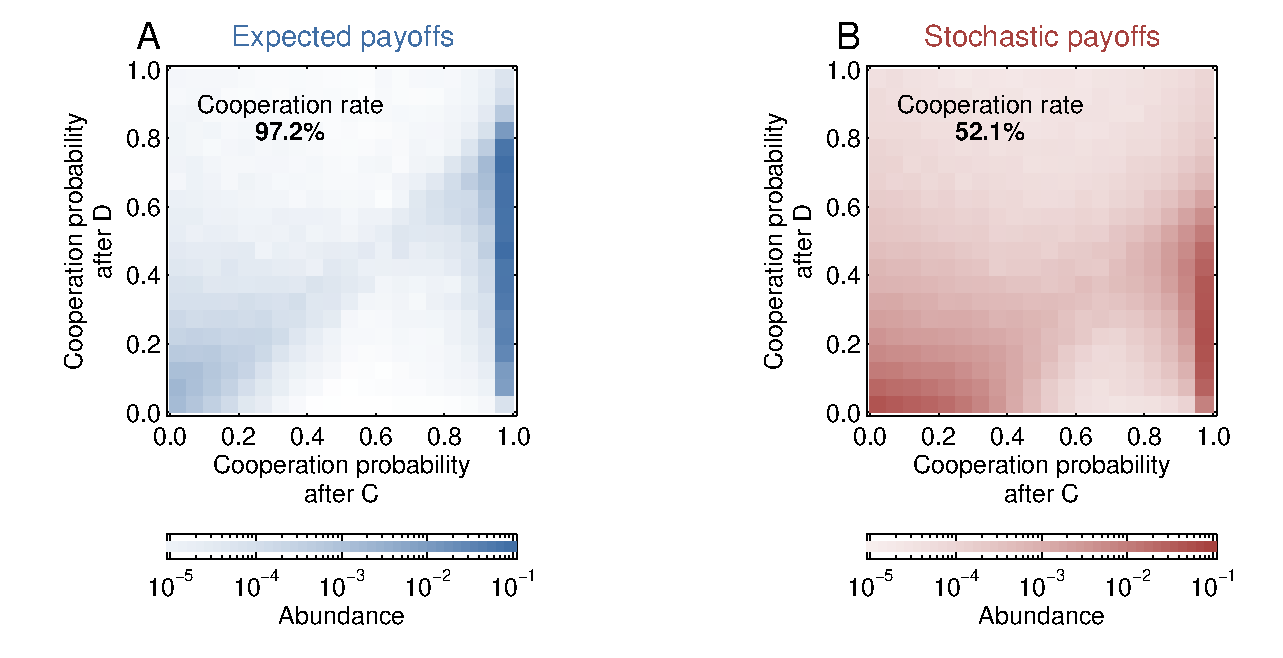
\includegraphics[width=0.75\textwidth]{Fig1} 
\caption{{\bf Evolutionary dynamics under expected payoffs (left) and stochastic payoffs (right).} 
We have run two simulations of the evolutionary process described in Section~\ref{Sec:BasicSetup} for $T\!=\!10^7$ time steps. For each time step, we have recorded the current resident population ($y,p,q$). Since simulations are run for a relatively high continuation probability of $\delta\!=\!0.999$, we do not report the players' initial cooperation probability $y$. The graphs show how often the resident population chooses each combination ($p,q$) of conditional cooperation probabilities in the subsequent rounds. ({\bf A}) If players update based on their expected payoffs, the resident population typically applies a strategy for which $p\!\approx\!1$ and $q\!\le\!1\!-\!c/b\!=\!0.9$. The cooperation rate within the resident population (averaged over all games and over all time steps) is close to 100\%. ({\bf B}) When players update their strategies based on their realized payoffs in the last round, there are two different predominant behaviors. The resident population either consists of defectors (with $p\!\approx\!q\!\approx\!0$) or of conditional cooperators. In the latter case, the maximum level of $q$ consistent with stable cooperation is somewhat smaller compared to the expected-payoff setting, $q\!<\!0.5$. Also the resulting cooperation rate is smaller. On average, players cooperate roughly in half of all rounds. Parameters: $N\!=\!100$, $b\!=\!3$, $c\!=\!1$, $\beta\!=\!1$, $\delta\!=\!0.999$.}
\end{figure}

To obtain some intuition for this result, we have recorded which mutant strategies typically invade into an ALLD population, and which mutants invade into a GTFT population, for each of the two scenarios (\FigInvAnalysis). Compared to expected-payoff updating, the stochastic scenario drastically reduces the stability of GTFT. On average, it takes fewer mutants until a GTFT population is successfully invaded. Moreover, successful mutants  tend to be less cooperative. 

\begin{figure}[t!]
\centering
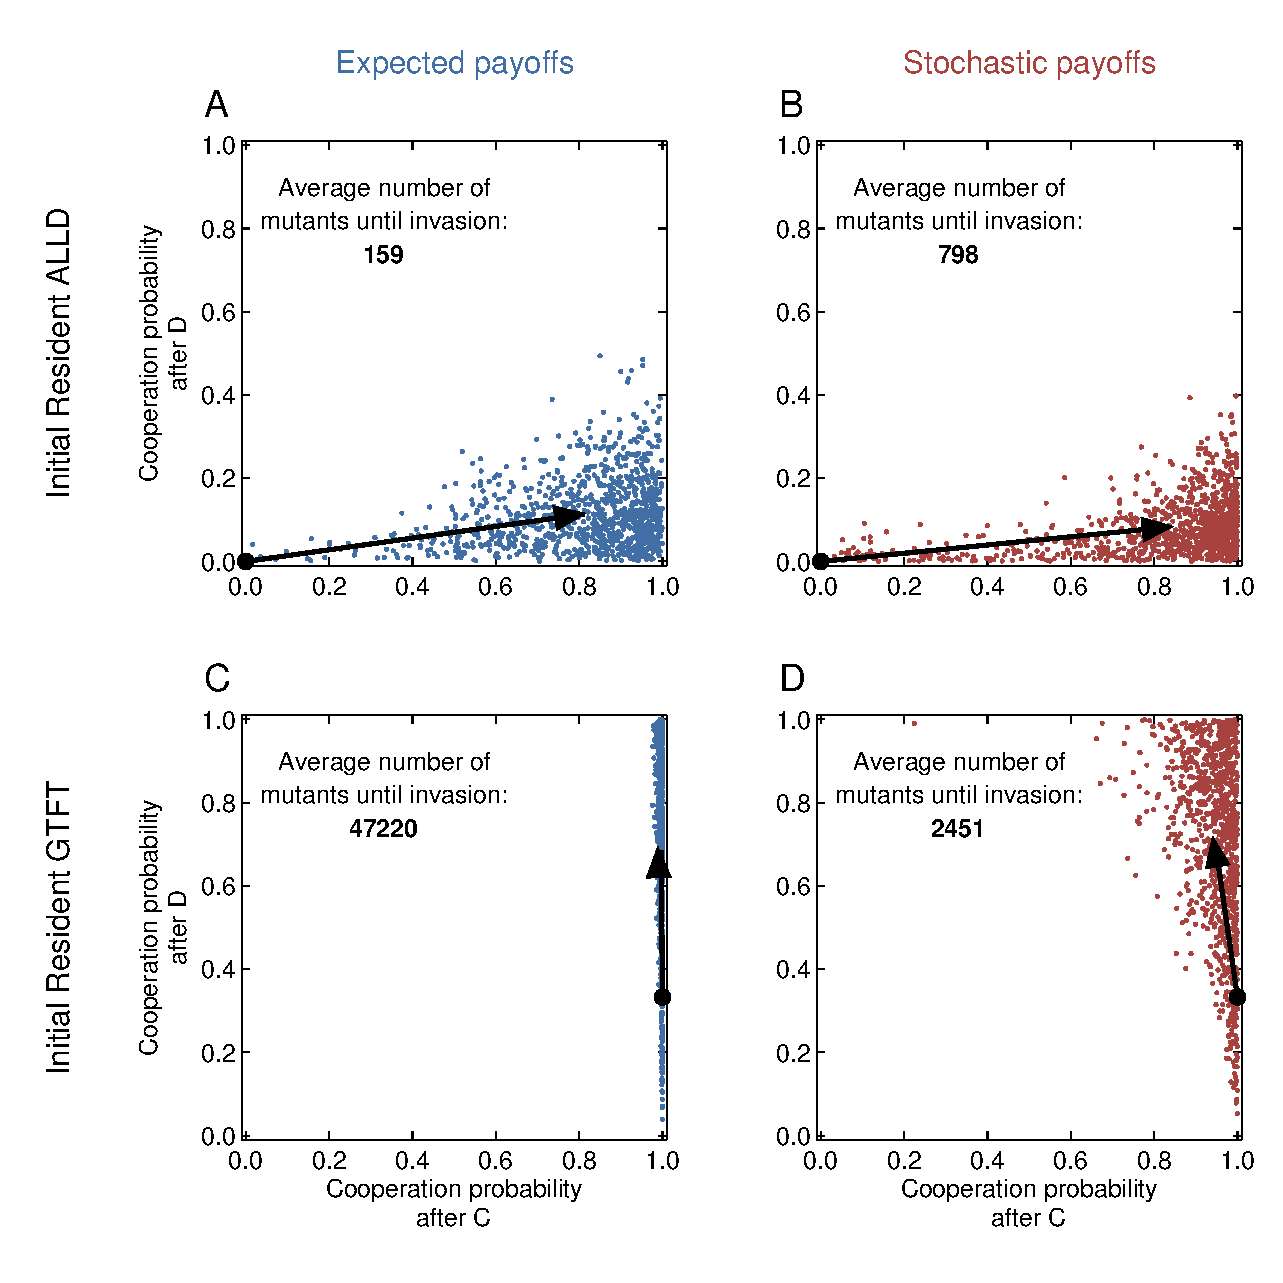
\includegraphics[width=0.75\textwidth]{Fig2} ~\\[-0.6cm]
\caption{{\bf Invasion into ALLD and into GTFT for the two evolutionary scenarios.} 
For this figure, we either consider a resident population of ALLD players (top) or of GTFT players (bottom). In each case, we have run 1,000 independent simulations of the evolutionary process described in Section~\ref{Sec:BasicSetup}. The colored dots within the four panels depict which mutant strategies successfully invaded into the respective resident population. The black arrow indicates the average over all successful mutant strategies. In addition, we have recorded how many mutant strategies need to be introduced into the population until the resident becomes replaced. Stochastic payoffs tend to increase the time until ALLD is invaded, and they reduce the time until GTFT is invaded. Parameters are the same as in \FigEvoProc. Strategies are defined as $ALLD\!=\!(0,0,0)$ and $GTFT=(1,1,1/3)$.}
~\\[0.4cm]
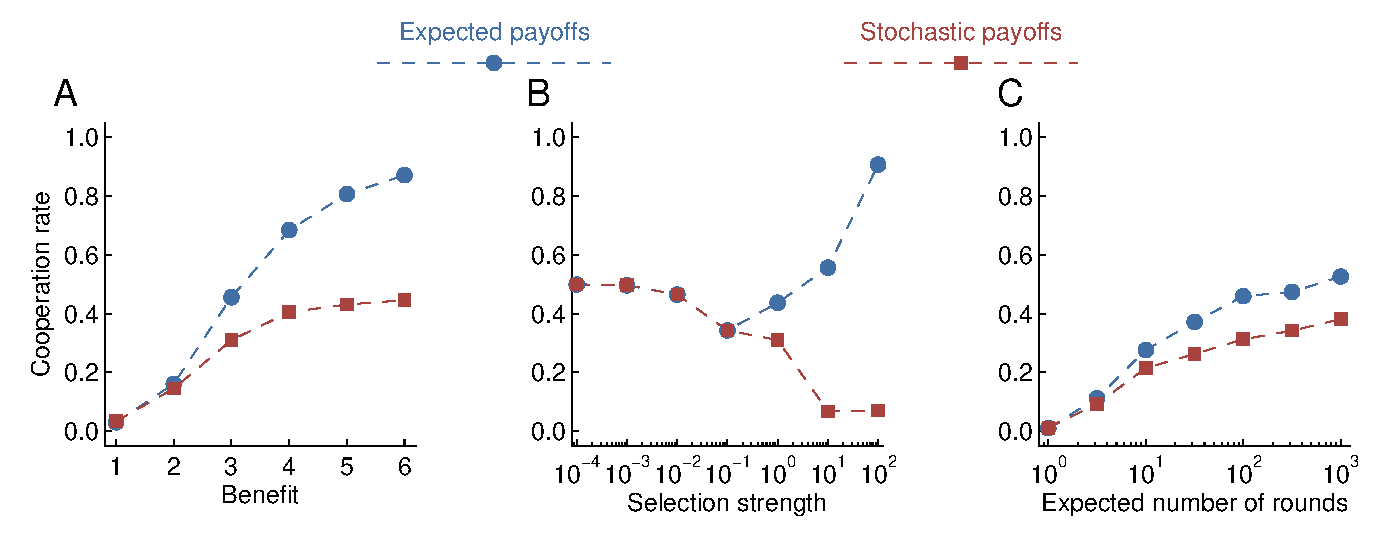
\includegraphics[width=0.8\textwidth]{Fig3} 
\caption{{\bf The evolution of cooperation for different parameter values.} 
While the previous figures depict the evolutionary outcome for fixed parameter values, here we vary the benefit of cooperation $b$, the strength of selection $\beta$, and the expected number of rounds, $1/(1\!-\!\delta)$. In all cases, stochastic payoff evaluation tends to reduce the evolving cooperation rates. Unless explicitly varied, the parameters of the simulation are $N\!=\!100$, $b\!=\!3$, $c\!=\!1$, $\beta\!=\!1$, $\delta\!=\!0.99$. Simulations are run for $T\!=\!5\times 10^6$ time steps for each parameter combination.}
\end{figure}

Finally, we have also explored how the evolving cooperation rates change as we vary the benefit $b$, the selection strength $\beta$, and the discount factor $\delta$ (\FigResultsOverPara). In all three cases, we find that the two scenarios yield similar cooperation rates when the respective parameters are small. Once there is a high benefit to cooperation, strong selection, or a high expected number of rounds, updating based on expected payoffs yields higher cooperation rates.

\clearpage
\newpage





{\setlength{\bibsep}{0\baselineskip} \small
\bibliographystyle{unsrt}
\input{bibliography.bbl}



\end{document}
